\section{Physikalische Grundlagen}

\subsection{Radioaktiver Zerfall}
\subsubsection{Das Zerfallsgesetz}
Für die Beschreibung des radioaktiven Zerfalls eines Isotops werden seine mittlere Lebensdauer $\tau$ 
und die Zerfallskonstante $\lambda =\frac{1}{\tau}$ verwendet.
Das Produkt $\lambda \cdot dt$ gibt die Wahrscheinlichkeit dafür an, dass ein Kern in der Zeiteinheit $dt$ zerfällt.
Aus der Halbwertszeit $T_{1/2}$ des Elements wird $\lambda$ so berechnet:
\begin{equation}
	\lambda=\frac{\ln (2)}{T_{1/2}}
\end{equation}
Das Produkt aus Zerfallskonstante und Zahl der vorhandenen Kerne $N(t)$ liefert die
Änderung der Kernanzahl $\frac{-d N(t)}{dt}$ und wird als Aktivität $A(t)$ bezeichnet:
\begin{equation}
	A(t)=\lambda N(t)= -\frac{d N(t)}{dt}
\end{equation}
Als Lösung dieser Differenzialgleichung erhält man das Zerfallsgesetz (mit $N_0 = N(0)$):
\begin{equation}
	N(t)=N_0 e^{-\lambda t}
\end{equation}
Damit erhält man für die Aktivität $A(t)$
\begin{equation}
	A(t)=\lambda N_0 e^{-\lambda t}
\end{equation}
Für lange Halbwertszeiten sind Kernanzahl $N$ und Aktivität $A$ nahezu konstant und es gilt
\begin{equation}
	A=\lambda N
\end{equation}

\subsubsection{$\alpha$-Zerfall}
Der $\alpha$-Zerfall findet nach folgendem Schema statt:
\begin{center}
${}^{A}_{Z}\text{X} \rightarrow {}^{A-4}_{Z-2}\text{Y} + {}^{4}_{2}\text{He}$
\end{center}
Der Mutterkern X mit Protonenzahl Z und Nukleonenzahl A zerfällt unter Aussendung eines Helium-Kerns
in den Tochterkern Y.
Der Zerfall findet statt, wenn der Helium-Kern durch den Coulomb-Wall des Mutterkerns tunnelt.\\
\chemel{Uran}{238} und \chemel{Samarium}{147} sind $\alpha$-Strahler:
\chemel{U}{238} zerfällt zu \chemel{Th}{234}, das ebenfalls nicht stabil ist.
Die Energie des ausgesendeten He-Kerns beträgt ca. 4\,MeV.
\chemel{Sm}{147} zerfällt zum stabilen \chemel{Nd}{143}, die Energie beträgt hier ca. 2\,MeV.

\subsubsection{$\beta$-Zerfall}
Beim $\beta^-$-Zerfall zerfällt ein Neutron im Kern zu einem Proton, einem Elektron und einem
Antielektronenneutrino:
\begin{center}
$\text{n} \rightarrow \text{p}^+ + \text{e}^- +\bar{\nu_e}$ bzw.\\[0.15cm]
${}^{A}_{Z}\text{X} \rightarrow {}^{A}_{Z+1}\text{Y} + \text{e}^- + \bar{\nu_e}$
\end{center}
Da beim Zerfall der Impuls unterschiedlich zwischen Elektron und Antineutrino aufgeteilt werden kann,
besitzt $\beta$-Strahlung ein kontinuierliches Energiespektrum, im Gegensatz zum diskreten Spektrum
bei $\alpha$-Strahlung.\\
Der $\beta^-$-Zerfall tritt bei \chemel{K}{40}-Kernen auf.
Sie zerfallen mit einer Wahrscheinlichkeit von 89.28\,\% zu \chemel{Ca}{40},
die Energie der Elektronen beträgt hier maximal 1.3\,MeV.\\
Auch \chemel{Th}{234}, das beim $\alpha$-Zerfall von \chemel{U}{238} entsteht,
zerfällt durch $\beta^-$-Zerfall zu Protaktinium \chemel{Pa}{234},
mit einer Energie der Elektronen von maximal 0.2\,MeV.

\subsubsection{Elektroneneinfang}
Die andere Zerfallsmöglichkeit von \chemel{K}{40} ist der Einfang eines inneren Schalenelektrons
in den Kern und Umwandlung eines Protons in ein Neutron:
\begin{center}
$\text{p}^+ + \text{e}^- \rightarrow \text{n} + \nu_e$ bzw.\\[0.15cm]
${}^{A}_{Z}\text{X} \rightarrow {}^{A}_{Z-1}\text{Y} + \nu_e$
\end{center}
Für \chemel{K}{40} bedeutet das eine Umwandlung zu \chemel{Ar}{40}.\\
Die Zerfallskonstanten für die beiden Zerfallsprozesse von \chemel{K}{40} addieren sich.
Da nur der $\beta^-$-Zerfall detektiert werden kann, muss dies bei der Bestimmung der
Halbwertszeit berücksichtigt werden.

\subsection{Absorption von radioaktiver Strahlung}

\subsection{Funktionsweise des Zählrohrs}

\begin{figure}[H]
\begin{center}
  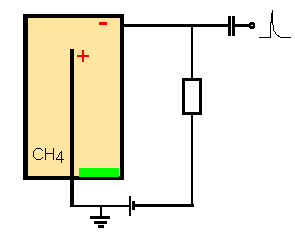
\includegraphics[width=8cm]{../img/aufbau}
  \caption[Zählrohrcharakteristik mit \uran]{Methangaszählrohr zur Bestimmung der Aktivität von radioaktiven Proben}
  \label{img:aufbau}
\end{center}
\end{figure}

\autoref{img:aufbau} zeigt den Aufbau des verwendeten Zählrohrs:
In einer mit Methan gefüllten Kammer befindet sich ein Draht auf Massepotential. Die Außenfläche der Kammer liegt auf einem
stark negativen Potential. Fliegt nun ein hochenergetisches Teilchen durch das Zählgas, werden Gasmoleküle ionisiert.
Bei einer geringen Zählrohrspannung rekombinieren die Ionen wieder mit ihren Elektronen.
Wird die Spannung erhöht, so gelangen positive Ionen bis zur Außenhülle und Elektronen an den Draht.
Ein Spannungspuls kann dann am Koppelungskondensator gemessen werden.
Eine weitere Erhöhung der Spannung führt zu einer sehr starken Beschleunigung der Elektronen im Feld nahe am Draht.
Diese schnellen Elektronen können weitere Gasmoleküle ionisieren. Aufgrund dieser Gasverstärkung
ist die Anzahl der erzeugten Ionen-Paare dann proportional zur Energie des einfallenden Teilchens.
In diesem Spannungsbereich werden die Experimente durchgeführt.\\
Bei sehr hoher Spannung geht die Verstärkung in Sättigung: Die Anzahl der erzeugten Ionen ist
für alle Teilchen unabhängig von ihrer Energie gleich hoch. Man spricht dann von einem Geiger-Müller-Zählrohr.


\subsection{Fehlerrechnung bei Zählraten}

Ist der Zerfälle $N$ pro Zeitintervall $t_n$ bekannt, so
beträgt die Zerfallsrate $n$
\begin{equation}
	n=\frac{N}{t_n}
\end{equation}
Da der radioaktive Zerfall poissonverteilt ist, gilt für den Fehler $s_N$ auf $N$
\begin{equation}
	s_N=\sqrt{N}
\end{equation}
Mit dem Gaußschen Fehlerfortpflanzungsgesetz erhält man für den Fehler der Zerfallsrate
\begin{equation}
	s_{n}=
	\sqrt{\left(\frac{\partial }{\partial N}\frac{N}{t_n}\right)^2 \cdot s_N{}^2}=
	\frac{s_N}{t_n}=
	\frac{\sqrt{N}}{t_n}=
	\frac{\sqrt{n \cdot t_n}}{t_n}=
	\sqrt{\frac{n}{t_n}}
\end{equation}
Für den relativen Fehler $s_{n,\text{rel}}$ erhält man damit
\begin{equation}
	s_{n,\text{rel}}=\frac{s_{n}}{n}=
	\frac{1}{\sqrt{n \cdot t_n}}
\end{equation}
bzw.
\begin{equation}
\label{eq:messzeit}
	t_n=
	\frac{1}{n \cdot s_{n,\text{rel}}{}^2}
\end{equation}

Meist ist es nicht möglich, die Zählrate $n$ direkt zu messen, da zusätzlich noch eine Untergrundstrahlung
vorhanden ist. Die gemessene Zählrate $\hat{n}$ muss also um die Untergrundzählrate $u$ bereinigt werden:
\begin{equation}
   n = \hat{n} - u
\end{equation}
Man erhält dann für den Fehler $s_n$
\begin{equation}
  s_n=\sqrt{s_{\hat{n}}{}^2+s_u{}^2}=\sqrt{\frac{\hat{n}}{t_{\hat{n}}}+\frac{u}{t_u}}
\end{equation}
